\documentclass[hidelinks,10pts]{article}
\usepackage[export]{adjustbox}
\usepackage{amsmath}
\usepackage{amssymb}
\usepackage[title,titletoc]{appendix}
\usepackage{array}
\usepackage[english]{babel}
\usepackage{bbm}
\usepackage{blindtext}
\usepackage{bookmark}
\usepackage{booktabs}
\usepackage{cancel}
\usepackage{caption}
\usepackage{csquotes}
\usepackage{enumerate}
\usepackage{enumitem}
\usepackage{epigraph}
\usepackage[left]{eurosym}
\usepackage{float}
\usepackage[bottom]{footmisc}
\usepackage[margin=0.9in]{geometry}
\usepackage{graphicx}
\usepackage{hyperref}
\usepackage{indentfirst}
\usepackage{listings}
\usepackage{lscape}
\usepackage{mathtools}
\usepackage{mdframed}
\usepackage{multirow}
\usepackage{multicol}
\usepackage[sort]{natbib}
\usepackage{parskip}
\usepackage{setspace}
\usepackage{subcaption}
\usepackage{titlesec}
\usepackage{tgpagella}
\usepackage{varwidth}
\usepackage{verbatim} %comment block
\usepackage{wrapfig}
\usepackage[dvipsnames]{xcolor}
\usepackage{xltabular}

\renewcommand{\epigraphsize}{\normalsize}
\setlength{\epigraphwidth}{0.7\textwidth}
\renewcommand{\textflush}{flushright}
\renewcommand{\sourceflush}{flushright}


\renewcommand\appendixpagename{Mathematical Appendix}
\renewcommand{\baselinestretch}{1.45}

\hypersetup{
    colorlinks=true, 
    urlcolor= Violet, 
    linkcolor=Violet, 
    citecolor=Blue, 
    filecolor = Blue
    } 

%\usepackage{natbib}
\bibliographystyle{plainnat}
%\bibdata{My Library.bib}
%\usepackage[backend=biber, style=authoryear-icomp]{biblatex}

\DeclareMathOperator{\E}{\mathbb{E}}
\DeclareMathOperator{\Prb}{\mathbb{P}}
\DeclareMathOperator{\R}{\mathbb{R}}
\DeclareMathOperator{\N}{\mathbb{N}}
\DeclareMathOperator{\1}{\mathbbm{1}}
\newcommand{\ind}{\perp\!\!\!\!\perp}


\titleformat{\part}{\centering\normalfont\Large\bfseries}{\partname\hspace{5pt}\thepart\hspace{5pt}}{5pt}{--\ }

\titleformat{\part}{\centering\normalfont\Large\bfseries}{\partname\hspace{5pt}\thepart\hspace{5pt}}{5pt}{--\ }

\makeatletter
\def\@fnsymbol#1{\ensuremath{\ifcase#1\or \dagger\or \ddagger\or
   \mathsection\or \mathparagraph\or \|\or **\or \dagger\dagger
   \or \ddagger\ddagger \else\@ctrerr\fi}}
    \makeatother

%code snippets 
\definecolor{codegreen}{rgb}{0,0.6,0}
\definecolor{codegray}{rgb}{0.5,0.5,0.5}
\definecolor{codepurple}{rgb}{0.58,0,0.82}
\definecolor{backcolour}{rgb}{0.95,0.95,0.92}

\lstdefinestyle{mystyle}{
    backgroundcolor=\color{backcolour},   
    commentstyle=\color{codegreen},
    keywordstyle=\color{magenta},
    numberstyle=\tiny\color{codegray},
    stringstyle=\color{codepurple},
    basicstyle=\ttfamily\footnotesize,
    breakatwhitespace=false,         
    breaklines=true,                 
    captionpos=b,                    
    keepspaces=true,                 
    numbers=left,                    
    numbersep=5pt,                  
    showspaces=false,                
    showstringspaces=false,
    showtabs=false,                  
    tabsize=2
}

\lstset{style=mystyle}





\begin{document}

        \title{\scshape{Asset Pricing - Empirical Application 1\\Factorial Model and Risk Premium Decomposition - APT }}%Arbitrage Pricing Theory: Decomposition of the Risk Premium}}
        \author{Luis Miguel Fonseca \\ Stéphane Eloundou Mvondo\\ Natalia Cárdenas Frías }
        \date{\today}
        \maketitle 


% an example of a factorial model including exogenous and endogenous factors based on the APT approach proposed by Ross; refer also to Fama and French factors

%In this application we apply Ross 1976 Arbitrage Theory Pricing (ATP) to decompose the risk premium of a stock index, the DAX40, using the multibeta relationship. 
%This is meant to better understand the returns of the assets by identifying the market price of risk and the factors that contribute to it. 

\section*{Introduction}

Focusing on recent data from the French equity market, we want to better comprehend how the market prices systemic, non-diversifiable risk embedded in the risk premium of stocks, i.e. any expected compensation beyond the risk-free return.
We base our analysis on a linear decomposition of said premium on different \emph{factors} of risk in the spirit of the Arbitrage Pricing Theory (APT) pioneered by \cite{rossArbitrageTheoryCapital1976}. 
Unlike the CAPM model which considers a unique risk premium in the market, the Ross model gives a more detailed description of the pricing of aggregate risk by decomposing the contributions of different sources of risk. 
Here, a risky portfolio of $j$ stocks\footnote{Let $j \in \{1,...,J\}$ with $J$ sufficiently large so that all idiosyncratic risk can be fully diversified. We better explain the difference between idiosyncratic and aggregate in the context of the Ross model in Section \ref{sec:model}} is compensated with  $k$ risk premia associated with the $k$ \emph{common factors} that the portfolio is exposed to.

\begin{comment}
\emph{factors} of aggregate risk is compensated by $k$ 
of the risk premium by identifying the compensation of $k$ different 


Unlike the CAPM model that considers a unique risk premium, the factorial model considers that investors holding risk in their portfolios\footnote{We assume that said portfolios are sufficiently large so that any source of idiosyncratic risk can be diversified so that only aggregate risk is remunerated.} by holding a stock $j$, are compensated with $k$ different risk premia associated to $k$ common factors.% which impact the returns of every stock, potentially in different manners. 

\end{comment}





\section{Data} 

    \subsection{French stock market data} \label{sec:model}
We decided to build a case study of the French market because it is a liquid and matured market, central in Europe. 
In the case of this analysis, we had trouble getting the data needed to perform it for other countries\footnote{Initially we thought about using data from the German market but we couldn't for instance find data for their inflation-linked bond yield that we use as an endogenous factor in Section \ref{sec:endofact}} and the fact that France has more publicly available data helped us choose it as our market of study. 

We built a portfolio with 30 French stocks that we got from Yahoo Finance. 
For simplicity, the synthetic portfolio is composed of one stock of each company and its composition does not change during the period studied.
Table \ref{tab:companies} shows the companies that we used to create this portfolio, they are all publicly traded companies in France since the early 2000's in Euronext Paris.
Importantly, we tried to have a certain diversity in the sectors represented to be able to capture some diversification to risk even if the portfolio is too small and we do not reweight it. 
However, because we try to implement a version of the \cite{famaCrossSectionExpectedStock1992} factor analysis, we restrain ourselves from choosing financial companies as the authors do due to their high leverage. 
Other than these two conditions, the choice of the companies was mainly restricted to data availability on public 'long' series on firm-level data, notably on market capitalization and book-to-market ratio to be able to incorporate the \cite{famaCrossSectionExpectedStock1992} factors to our analysis. 

%\textcolor{red}{describe frequency of data }

Because we are interested in the underlying determinants of the risk premia, and due to data availability issues, we decided to have a broad analysis with monthly data for our selection of stocks for the period 2005-2022. 
Monthly data is for instance used by \cite{chenEconomicForcesStock1986}.
While this is not a very long period, it encompasses important moments in the financial markets in particular the Great Financial Crisis, the subsequent European Debt Crisis, and the Covid years. 
Also importantly, during most of this period (following the GFC), monetary policy fixed interest rates were extremely low driving down the return of sovereign debt for countries like France and Germany\footnote{They were negative for certain maturities in real terms for a part of the time frame analyzed, pretty much since the European Debt Crisis until the inflation surge after Covid.} that could have been assimilated to the risk-free rate. 
This means that for an investor to get any returns, it had to hold risky assets. 
Moreover, the period following the GFC and up to 2021 was also characterized by extremely low inflation in the Euro Zone. 
This is interesting because the APT usually incorporates inflation risk as market risk, yet inflation was nowhere to be found for more than a decade. 
Seeing how the market incorporated this monetary reality is by itself an intriguing question.


\begin{table}[h]
    \centering
    \begin{tabular}{|c|c|c|}
    \hline
    \textbf{Company Name} & \textbf{Ticker} & \textbf{Industry} \\
    \hline
Accor & AC.PA & Hospitality \\
Air Liquide & AI.PA & Industrial Gases \\
Air France-KLM & AF.PA & Airlines \\
Airbus & AIR.PA & Aerospace \\
Biomerieux & BIM.PA & Biotechnology \\
BIC & BB.PA & Consumer Goods \\
Bouygues & EN.PA & Construction \\
Capgemini & CAP.PA & Information Technology \\
Carrefour & CA.PA & Retail \\
Casino & CO.PA & Retail \\
Dassault Aviation & AM.PA & Aerospace \\
Danone & BN.PA & Food and Beverage \\
Hermes International & RMS.PA & Fashion and Luxury \\
JCDecaux & DEC.PA & Advertising \\
Kering & KER.PA & Fashion and Luxury \\
L'Oreal & OR.PA & Cosmetics \\
LVMH & MC.PA & Fashion and Luxury \\
Michelin & ML.PA & Automotive \\
Nexans & NEX.PA & Electrical Equipment \\
Orange & ORA.PA & Telecommunications \\
Renault & RNO.PA & Automotive \\
Saint-Gobain & SGO.PA & Manufacturing \\
Sanofi & SAN.PA & Pharmaceuticals \\
Sodexo & SW.PA & Food Services \\
TF1 & TFI.PA & Broadcasting \\
Thales & HO.PA & Aerospace and Defense \\
TotalEnergies & TTE.PA & Energy \\
Ubisoft & UBI.PA & Video Games \\
Vinci & DG.PA & Construction \\
Vivendi & VIV.PA & Entertainment \\
\hline
\end{tabular}
\caption{Synthetic portfolio: Companies, Tickers, and Industries}
\label{tab:companies}
\end{table}



\subsection{Data description and sources}
%We decided to take the components of the DAX 40 
The other series that we use are the following and its sources, how they are used in the context of the analysis is described in subsequent sections. %Due to data availability issues and time constraints, w

\begin{itemize}
    \item As a proxy for the free rate of the market we consider two measures: 
    \begin{itemize}
        \item The yield of short-term OAT, i.e. French treasuries taken from \hyperlink{https://www.banque-france.fr/fr/statistiques/taux-indicatifs-des-bons-du-tresor-et-oat-03-oct-2023-03-oct-2023}{Banque de France's website}. As for most developed, stable countries, short-term sovereign bonds are taken as the risk-free asset as Governments are supposed to be more solvent than other agents in the economy, after all, they decide their income and could seize resources via taxes to meet their obligations.        
        \item The spot yield curve spot rate, for 3-month maturity of all government bonds rated triple A in the Euro Area, retrieved from the \hyperlink{https://data.ecb.europa.eu/data/datasets/YC/YC.B.U2.EUR.4F.G_N_A.SV_C_YM.SR_3M?chart_props=W3sibm9kZUlkIjoiMTg5NTYzMSIsInByb3BlcnRpZXMiOlt7ImNvbG9ySGV4IjoiIiwiY29sb3JUeXBlIjoiIiwiY2hhcnRUeXBlIjoibGluZWNoYXJ0IiwibGluZVN0eWxlIjoiU29saWQiLCJsaW5lV2lkdGgiOiIxLjUiLCJheGlzUG9zaXRpb24iOiJsZWZ0Iiwib2JzZXJ2YXRpb25WYWx1ZSI6ZmFsc2UsImRhdGVzIjpbXSwiaXNUZGF0YSI6ZmFsc2UsIm1vZGlmaWVkVW5pdFR5cGUiOiIiLCJ5ZWFyIjoib25lIiwic3RhcnREYXRlIjoiMjAyMi0xMS0yMyIsImVuZERhdGUiOiIyMDIzLTExLTIzIiwic2V0RGF0ZSI6ZmFsc2UsInNob3dUYWJsZURhdGEiOnRydWUsImNoYW5nZU1vZGUiOmZhbHNlLCJzaG93TWVudVN0eWxlQ2hhcnQiOmZhbHNlLCJkaXNwbGF5TW9iaWxlQ2hhcnQiOnRydWUsInNjcmVlblNpemUiOiJtYXgiLCJzY3JlZW5XaWR0aCI6MTQ0MCwic2hvd1RkYXRhIjpmYWxzZSwidHJhbnNmb3JtZWRGcmVxdWVuY3kiOiJub25lIiwidHJhbnNmb3JtZWRVbml0Ijoibm9uZSIsImZyZXF1ZW5jeSI6Im5vbmUiLCJ1bml0Ijoibm9uZSIsIm1vZGlmaWVkIjoiZmFsc2UiLCJzZXJpZXNLZXkiOiJkYWlseSAtIGJ1c2luZXNzd2VlayIsInNob3d0YWJsZVN0YXRlQmVmb3JlTWF4U2NyZWVuIjpmYWxzZSwiaXNkYXRhY29tcGFyaXNvbiI6ZmFsc2UsInNlcmllc0ZyZXF1ZW5jeSI6ImRhaWx5IC0gYnVzaW5lc3N3ZWVrIiwiaW50aWFsU2VyaWVzRnJlcXVlbmN5IjoiZGFpbHkgLSBidXNpbmVzc3dlZWsiLCJtZXRhZGF0YURlY2ltYWwiOiI2IiwiaXNUYWJsZVNvcnRlZCI6ZmFsc2UsImlzWWVhcmx5VGRhdGEiOmZhbHNlLCJyZXNwb25zZURhdGFFbmREYXRlIjoiIiwiaXNpbml0aWFsQ2hhcnREYXRhIjp0cnVlLCJpc0RhdGVzRnJvbURhdGVQaWNrZXIiOmZhbHNlLCJkYXRlUGlja2VyRW5kRGF0ZSI6IiIsImlzRGF0ZVBpY2tlckVuZERhdGUiOmZhbHNlLCJzZXJpZXNrZXlTZXQiOiIiLCJkYXRhc2V0SWQiOiIxMjUiLCJpc0NhbGxiYWNrIjpmYWxzZSwiaXNTbGlkZXJUZGF0YSI6ZmFsc2UsImlzU2xpZGVyRGF0YSI6ZmFsc2UsImlzSW5pdGlhbENoYXJ0RGF0YUZyb21HcmFwaCI6ZmFsc2UsImNoYXJ0U2VyaWVzS2V5IjoiWUMuQi5VMi5FVVIuNEYuR19OX0EuU1ZfQ19ZTS5TUl8zTSIsInR5cGVPZiI6ImRvd25Mb2FkIn1dfV0\%3D}{ECB webpage}. On top of the fact that this is a measure for short-term sovereign bonds, we consider this to be a relevant proxy for the French market due to the strong integration within the European capital market. If an investor decides that the French market becomes risky, she can easily move her investments to another European capital market that looks safer. 
    \end{itemize}
    \item To get the market rate, we use the return of the main index of the country, the CAC40 also taken from Yahoo Finance as for the components of our synthetic portfolio. In hindsight, we are not sure of the pertinence of comparing our portfolio to this index. While the composition of our portfolio is not the same as the CAC40\footnote{Not all the stocks we chose are necessarily part of the CAC40 at every period studied, and the CAC40 is a weighted index that evolves over time.}, due to the data availability issues we've been mentioning, we see that our choices are heavily biased towards 'big name' companies that are those belonging to the index.
    \item We got the series of the exchange rate between the Euro and the US dollar from Yahoo Finance. It is read as the amount of USD needed to get one euro. 
    \item The GDP series is taken from the \hyperlink{https://data.ecb.europa.eu/data/datasets/MNA/MNA.Q.Y.FR.W2.S1.S1.B.B1GQ._Z._Z._Z.XDC.LR.N?chart_props=W3sibm9kZUlkIjoiNjEzMzI0IiwicHJvcGVydGllcyI6W3siY29sb3JIZXgiOiIiLCJjb2xvclR5cGUiOiIiLCJjaGFydFR5cGUiOiJsaW5lY2hhcnQiLCJsaW5lU3R5bGUiOiJTb2xpZCIsImxpbmVXaWR0aCI6IjEuNSIsImF4aXNQb3NpdGlvbiI6ImxlZnQiLCJvYnNlcnZhdGlvblZhbHVlIjpmYWxzZSwiZGF0ZXMiOlsiMjAwMC0wMy0wNFQyMzowMDowMC4wMDBaIiwiMjAyMy0wOS0yOVQyMjowMDowMC4wMDBaIl0sImlzVGRhdGEiOmZhbHNlLCJtb2RpZmllZFVuaXRUeXBlIjoiIiwieWVhciI6ImRhdGV3aXNlIiwic3RhcnREYXRlIjoiMjAwMC0wMy0wNSIsImVuZERhdGUiOiIyMDIzLTA5LTMwIiwic2V0RGF0ZSI6dHJ1ZSwic2hvd1RhYmxlRGF0YSI6ZmFsc2UsImNoYW5nZU1vZGUiOmZhbHNlLCJzaG93TWVudVN0eWxlQ2hhcnQiOmZhbHNlLCJkaXNwbGF5TW9iaWxlQ2hhcnQiOnRydWUsInNjcmVlblNpemUiOiJtYXgiLCJzY3JlZW5XaWR0aCI6MTQ0MCwic2hvd1RkYXRhIjpmYWxzZSwidHJhbnNmb3JtZWRGcmVxdWVuY3kiOiJub25lIiwidHJhbnNmb3JtZWRVbml0Ijoibm9uZSIsImZyZXF1ZW5jeSI6Im5vbmUiLCJ1bml0Ijoibm9uZSIsIm1vZGlmaWVkIjoiZmFsc2UiLCJzZXJpZXNLZXkiOiJxdWFydGVybHkiLCJzaG93dGFibGVTdGF0ZUJlZm9yZU1heFNjcmVlbiI6ZmFsc2UsImlzZGF0YWNvbXBhcmlzb24iOmZhbHNlLCJzZXJpZXNGcmVxdWVuY3kiOiJxdWFydGVybHkiLCJpbnRpYWxTZXJpZXNGcmVxdWVuY3kiOiJxdWFydGVybHkiLCJtZXRhZGF0YURlY2ltYWwiOiIyIiwiaXNUYWJsZVNvcnRlZCI6ZmFsc2UsImlzWWVhcmx5VGRhdGEiOmZhbHNlLCJyZXNwb25zZURhdGFFbmREYXRlIjoiMjAyMy0wOS0zMCIsImlzaW5pdGlhbENoYXJ0RGF0YSI6dHJ1ZSwiaXNEYXRlc0Zyb21EYXRlUGlja2VyIjp0cnVlLCJkYXRlUGlja2VyRW5kRGF0ZSI6IjIwMjMtMDktMzAiLCJpc0RhdGVQaWNrZXJFbmREYXRlIjp0cnVlLCJzZXJpZXNrZXlTZXQiOiIiLCJkYXRhc2V0SWQiOiIyNDkiLCJpc0NhbGxiYWNrIjpmYWxzZSwiaXNTbGlkZXJUZGF0YSI6dHJ1ZSwiaXNTbGlkZXJEYXRhIjp0cnVlLCJpc0luaXRpYWxDaGFydERhdGFGcm9tR3JhcGgiOnRydWUsImNoYXJ0U2VyaWVzS2V5IjoiTU5BLlEuWS5GUi5XMi5TMS5TMS5CLkIxR1EuX1ouX1ouX1ouWERDLkxSLk4iLCJ0eXBlT2YiOiIifV19XQ\%3D\%3D}{ECB webpage}. It is available at a quarterly frequency and is available at market prices. 
    \item The harmonized headline inflation rate is taken from the \hyperlink{https://www.insee.fr/fr/statistiques/serie/010576187}{INSEE webpage}. 
    \item For the market inflation expectation in a 10-year horizon, we use the break-even inflation rate published by \hyperlink{https://www.aft.gouv.fr/en/oateuroi-key-figures\#serie}{Agence France Trésor} online. Sadly, data is only available from 2013.
    \item For the implementation of the two additional \cite{famaCrossSectionExpectedStock1992} factors, we took different routes
    \begin{itemize}
        \item We found the estimation of the factors published by K. French in his \href{https://mba.tuck.dartmouth.edu/pages/faculty/ken.french/data_library.html}{online Data Library} that are constantly updated. Their estimations start in the 1990s and are made for different markets using the comprehensive CRSP dataset that is not freely available. He has an estimation for the European market that we downloaded to use but it is not clear which stocks are used to replicate their portfolio.
        \item To try to build these estimations ourselves for our portfolio meaning that a minima we need data on the market capitalization of each company during the time frame studied and its \emph{book}. This information is hardly available without having access to platforms like Bloomberg or CRSP. The best information that we could find comes from \href{https://companiesmarketcap.com/}{this} website that publishes the market capitalization and the price-to-book (the inverse of the book-to-market ratio) annual series for several stocks. The data is however cannot be directly downloaded from the site so we scrap it to get the series (see Code Appendix \ref{sec:datacode}). Our biggest fear with this source is that it is not clear at all where the information comes from even if they mention several quality \href{https://companiesmarketcap.com/stockmarket-api/}{data providers} as their partners. Since it is the only source that resembles what is needed for this part we used it but we are not confident about it. 
    \end{itemize}
\end{itemize}




\section{Empirical strategy and implementation}


%For the sake of completeness, this section summarizes the lecture on the \cite{rossArbitrageTheoryCapital1976} model and the multibeta relationship as they are the theoretical foundation of the empirical application.
We implement a minimal approach to \cite{rossArbitrageTheoryCapital1976}, namely using fewer factors than in \cite{chenEconomicForcesStock1986}. 
We include both exogenous and endogenous macroeconomic risk factors as well as an approximation to implement \cite{famaCommonRiskFactors1993} three-factor model which used stock-specific data. 

Let the return $R_j$ of the $j$-th component of her portfolio can be described by the following expression $\forall j\in \{1,...,N\}$: 
    \begin{equation} \label{eq:factorialmodel}
        R_j = \E[R_j] + \underbrace{\sum_{k=1}^K \beta_{j,k} f_k}_{\mathclap{\text{Systemic risk}}} + \overbrace{u_j}^{\mathclap{\text{Idiosyncratic risk}}}
    \end{equation}
Where $\E[R_j]$ is the expected return of asset $j$ and $R_j$ its return without dividend i.e. the first difference of the stock price. 
This is the so-called \emph{factorial model} that includes two sources of risk:
\begin{enumerate}
    \item[i.] The investor faces centered idiosyncratic risks $u_j$, $\E[u_j]=0$ that are assumed to be completely diversiable with a portfolio "large enough" ($N$ big) because they are independent of each other $u_j \ind u_{j'} \forall j\neq j' $.
    \item[ii.] She also faces $k$ different sources of aggregate risk, modeled by the linear combination of $f_k$ centered \emph{shocks} that influence all $R_j$ with a sensitivity $\beta_{jk}$. 
    By definition, these risks cannot be diversified because they affect the returns of all asset and thus has to be compensated which is the focal point of our study. 
\end{enumerate}
In order to implement a regression analysis and estimation as the one that follows in this section, we shall also assume that the idiosyncratic risks are uncorrelated with aggregate risk $corr(u_j, f_k) = 0, \forall j, k$.

This section is organized as follows. 
Section \ref{sec:identiffactors} identifies the aggregate market risks $(f_k)_k$ that we are going to consider as the ones priced by the market. 
Section \ref{sec:betas} runs a first regression analysis to identify the sensitivity of each return to each factor of risk, i.e. to identify the $(\beta_{j,k})_{j,k}$ from the factorial model(Eq. \ref{eq:factorialmodel}). It also implements an approximation to a parallel model that decomposes the return of stocks: the \cite{famaCrossSectionExpectedStock1992} that also will lead us to estimate the sensitivity of the return of each return to a series of factors. 
Finally, section \ref{sec:lambdas} uses the series of $(\hat{\beta}_{j,k})_{j,k}$ estimated before to implement an estimation of the \emph{multibeta relationship} which is the regression that will allow us to get how much the market is remunerating the exposition to a market factor risk.


    \subsection{Identify the risk factors} \label{sec:identiffactors}
We decided to explore the role of the following sources of risk for a first model inspired by \cite{rossArbitrageTheoryCapital1976} and \cite{chenEconomicForcesStock1986}.
\begin{itemize}
    \item The activity risk, measured by changes in GDP
    \item Inflation risk, measured both by the HICP of France for the short term and by the market inflation expectation in a 10-y horizon. 
    \item Devaluation risk measured by the exchange rate between the Euro and the US dollar.
\end{itemize}
We then consider the factors of a complementary factor model, \cite{famaCrossSectionExpectedStock1992} which are not directly linked to risks.

        \subsubsection{Exogeneous factors}
These are risk factors that do not depend directly on the financial markets or more precisely that are not deduced from a linear combination of the returns of financial assets.  
In our case, it is mainly the activity risk, the short-term interest rate (measured by the HICP), and the devaluation risk. 
Importantly, the measure of these risks is not directly measured by changes or by the level of the underlying variables as markets are informational efficient [Fama, 1970], and they have already priced in all relevant information conveyed by prices. 
In particular, all \emph{predictable} movements, say in inflation, have already been incorporated by the market. 
This means that the factors of risk are actually the \emph{surprises} in the movements of these variables. 

To extract this unpredictable part of these variables we need to use the residuals of some time series model of the (stationary) variables\footnote{Evidently, we need that the series used are stationary before conducting any TS analysis. We tested for stationarity of our series using the ADP test and then differentiate the series that were non-stationary (see Appendix \ref{sec:extra}). We didn't apply the ADF test to the series in logs afterward as the R function \emph{auto.arima} automatically differentiates the series $d$ times until they are stationary.}, in our case ARIMA$(p,d,q)$ models.
We used the function \emph{auto.arima} from the R \emph{forecasts} package that set de parameters optimally by minimizing the BIC between different specifications. 
We ended up with: 
\begin{itemize}
    \item[-] ARIMA(0,1,0) (i.e. a random walk\footnote{We do find this result 'weird' but didn't find any mistake in the code}) for the series of log GDP. 
    \item[-] ARIMA(0,1,1) for the exchange rate series. 
    \item[-] ARIMA(2,1,2) for the HICP series. 
\end{itemize}

We then stored the residuals of each one of these models and merge it in the data frame with the stock return 


        \subsubsection{Endogeneous factors} \label{sec:endofact}
These factors are linear combinations of the returns of financial assets. 
We used the \emph{Breakeven Inflation} at a 10-year horizon which is simply the yield difference between 10-y OATi 0.10\% (\emph{Obligatiosn Assimilables du Trésor}) indexed by the HICP and non-indexed 10-y OAT. 
This gap is assimilated to how markets price the possibility of having future inflation\footnote{Note that the Breakeven inflation is the inflation rate that would equalize the return of these two sovereign bonds (due to AOA).}. 
Once again we need to extract the unforecastable movements in this indicator to have an adequate measure of risk. 
We follow the same methodology as with the exogenous factors and retrieve the residuals of an ARIMA(2,1,2) model.


        \subsubsection{French-Fama factors}

\cite{famaCommonRiskFactors1993} can also be seen as an extension of the CAPM model but their factors, while significant specially in the US market, are hardly interpretable as risk factors.
The authors show that the variation of the returns of an asset can be explained not only by the exposure to market risk as in the CAPM represented by the difference of the market return and the risk-free rate $[R_M-R_f]$, but also by a size and value premium in the following model.
    
    \begin{equation}
        R_j = \alpha_j + R_f + \beta_{m,j}[R_M-R_f] +\beta_{S} SMB + \beta_{V}HML +\varepsilon_j
    \end{equation}

The size premium refers to the observation that stocks with small market capitalizations tend to outperform stocks with larger ones and it is captured by the factor SMB, \emph{small minus big}.
It is computed as the difference in average returns of the $30\%$ stocks with the smallest market capitalization and the average returns of the $30\%$ stocks associated with the firms with the largest market capitalization. 
The value premium refers to the outperformance of "value stocks" i.e. those that have high book-to-market (B/M) and it is represented by the difference in an average return of the $50\%$ of stocks with the highest $B/M$ ratio (value stocks) and the $50\%$ with lowest $B/M$ ratio (growth stocks). 
We use this methodology to create our own SMB and HML factors at a yearly frequency. 

As we previously mentioned, K. French made public his estimation of the factors for the European model using a more complex approach with "6 value-weight portfolios formed on size and book-to-market". 
SMB (Small Minus Big) is the average return on the three small portfolios minus the average return on the three big portfolios, and HML (High Minus Low) is the average return on the two value portfolios minus the average return on the two growth portfolios. 





\begin{comment}
    
    The Fama/French factors are constructed using the 6 value-weight portfolios formed on size and book-to-market. (See the description of the 6 size/book-to-market portfolios.)
    
    SMB (Small Minus Big) is the average return on the three small portfolios minus the average return on the three big portfolios,
    
    
    SMB = 1/3 (Small Value + Small Neutral + Small Growth) - 1/3 (Big Value + Big Neutral + Big Growth).	 
    
    HML (High Minus Low) is the average return on the two value portfolios minus the average return on the two growth portfolios,
    
    
    HML = 1/2 (Small Value + Big Value) - 1/2 (Small Growth + Big Growth).	 
    
    Rm-Rf, the excess return on the market, value-weight return of all CRSP firms incorporated in the US and listed on the NYSE, AMEX, or NASDAQ that have a CRSP share code of 10 or 11 at the beginning of month t, good shares and price data at the beginning of t, and good return data for t minus the one-month Treasury bill rate (from Ibbotson Associates).
    
    See Fama and French, 1993, "Common Risk Factors in the Returns on Stocks and Bonds," Journal of Financial Economics, for a complete description of the factor returns.
\end{comment}


    \subsection{Estimate the sentitivities of the factorial model} \label{sec:betas}
%$\beta_k$ coefficients from the factorial model

\subsection{Ross model}
Given that we assumed that the idiosyncratic risks $u_j$



\section{French and Fama model}



    \subsection{Estimate the remuneration of risk from the multibeta relationship} \label{sec:lambdas}
%he $\lambda_k$ parameters

Under AOA, assuming that the factorial model (Eq. \ref{eq:factorialmodel}) is an accurate depiction of how equity is price, implies that the expected returns are constrained by a multibeta relationship of the following form $\exists \rho, \exists \lambda_1, ..., \lambda_k$: 
    \begin{equation}
        \E[R_j] = \rho + \sum^K_k=1 \lambda_k \beta_{j,k}
    \end{equation}
where each $\lambda_k$ is the parameter representing the market price of risk (the risk premium) that the market retributes for being exposed to a given risk factor $f_k$ with a sensitivity $\beta_{j,k}$%risk premium associated to the




    \subsection{Test the validity of the multibeta relationship}


    \subsection{Application of the French-Fama model}

\section*{Conslusion}

\newpage
\begin{appendices}
    \section{Additional tables and figures } \label{sec:extra}
\subsection*{Macroeconomic factors}


% Table created by stargazer v.5.2.3 by Marek Hlavac, Social Policy Institute. E-mail: marek.hlavac at gmail.com
% Date and time: Tue, Nov 28, 2023 - 19:23:43
\begin{table}[!htbp] \centering 
  \caption{Results ADF with trend and drift} 
  \label{} 
\begin{tabular}{@{\extracolsep{5pt}} cccccccccc} 
\\[-1.8ex]\hline 
\hline \\[-1.8ex] 
 & EuroUSD & CAC40 & Inflation & PIB & RF AAA & OAT & 1pct & 5pct & 10pct \\ 
\hline \\[-1.8ex] 
tau3 & $$-$2.945$ & $$-$2.028$ & $$-$0.565$ & $$-$4.716$ & $$-$1.011$ & $$-$0.720$ & $$-$3.990$ & $$-$3.430$ & $$-$3.130$ \\ 
phi2 & $3.012$ & $1.652$ & $1.243$ & $7.665$ & $0.800$ & $0.555$ & $6.220$ & $4.750$ & $4.070$ \\ 
phi3 & $4.421$ & $2.220$ & $1.522$ & $11.121$ & $1.198$ & $0.683$ & $8.430$ & $6.490$ & $5.470$ \\ 
\hline \\[-1.8ex] 
\end{tabular} 
\end{table} 


% Table created by stargazer v.5.2.3 by Marek Hlavac, Social Policy Institute. E-mail: marek.hlavac at gmail.com
% Date and time: Tue, Nov 28, 2023 - 19:32:21
\begin{table}[!htbp] \centering 
  \caption{Results ADF with drift} 
  \label{} 
\begin{tabular}{@{\extracolsep{5pt}} cccccccccc} 
\\[-1.8ex]\hline 
\hline \\[-1.8ex] 
& EuroUSD & CAC40 & Inflation & PIB & RF AAA & OAT & 1pct & 5pct & 10pct \\ 
% & statistic & statistic.1 & statistic.2 & statistic.3 & statistic.4 & statistic.5 & 1pct & 5pct & 10pct \\ 
\hline \\[-1.8ex] 
tau2 & $$-$1.841$ & $$-$1.428$ & $$-$0.444$ & $$-$2.117$ & $$-$1.545$ & $$-$1.142$ & $$-$3.460$ & $$-$2.880$ & $$-$2.570$ \\ 
phi1 & $1.791$ & $1.277$ & $0.438$ & $2.589$ & $1.195$ & $0.803$ & $6.520$ & $4.630$ & $3.810$ \\ 
\hline \\[-1.8ex] 
\end{tabular} 
\end{table} 


% Table created by stargazer v.5.2.3 by Marek Hlavac, Social Policy Institute. E-mail: marek.hlavac at gmail.com
% Date and time: Tue, Nov 28, 2023 - 19:32:35
\begin{table}[!htbp] \centering 
  \caption{Results ADF with no trend nor drift} 
  \label{} 
\begin{tabular}{@{\extracolsep{5pt}} cccccccccc} 
\\[-1.8ex]\hline 
\hline \\[-1.8ex] 
& EuroUSD & CAC40 & Inflation & PIB & RF AAA & OAT & 1pct & 5pct & 10pct \\ 
%& statistic & statistic.1 & statistic.2 & statistic.3 & statistic.4 & statistic.5 & 1pct & 5pct & 10pct \\ 
\hline \\[-1.8ex] 
tau1 & $$-$0.618$ & $0.414$ & $0.353$ & $0.721$ & $$-$1.437$ & $$-$0.995$ & $$-$2.580$ & $$-$1.950$ & $$-$1.620$ \\ 
\hline \\[-1.8ex] 
\end{tabular} 
\end{table} 


        \begin{figure}[h]
            \centering
            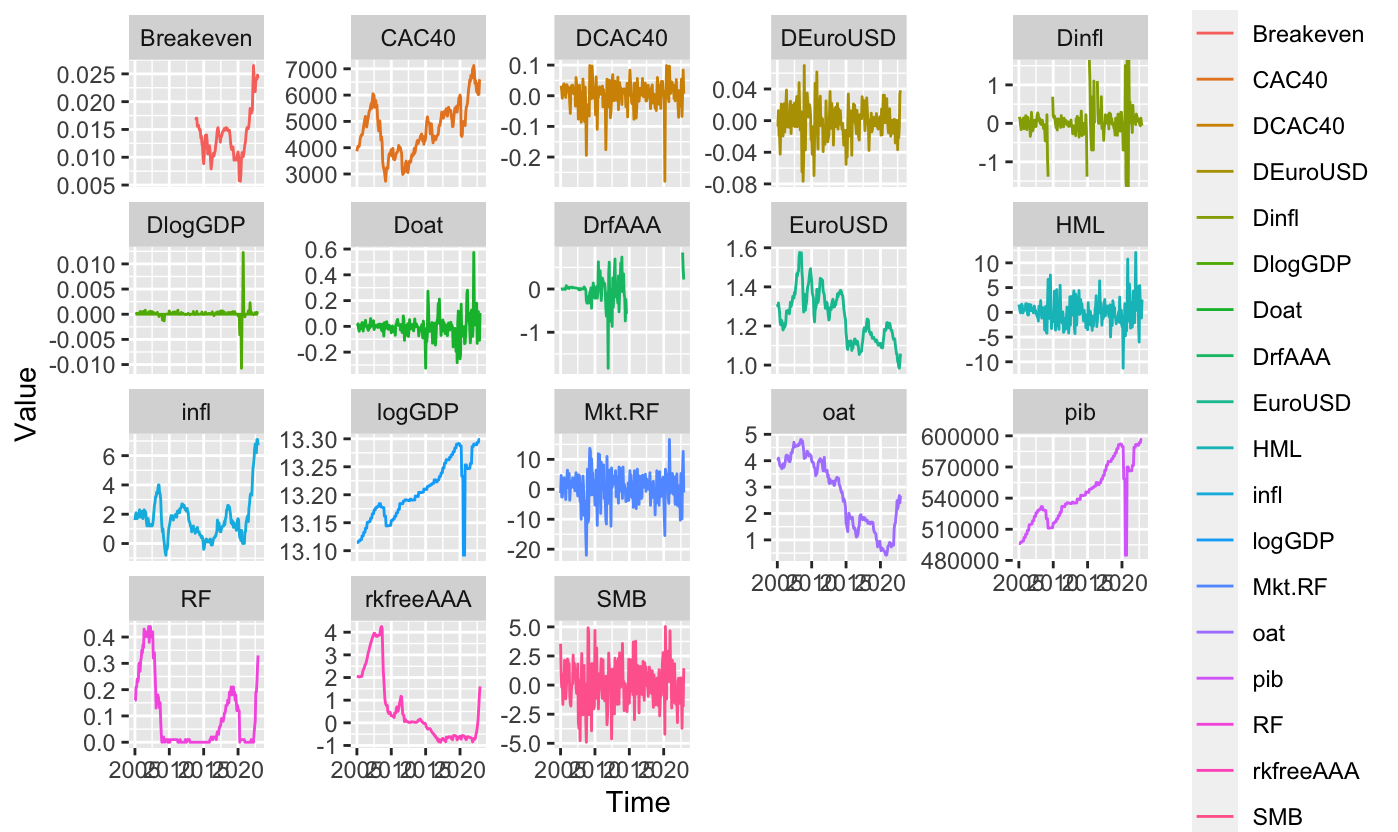
\includegraphics[width=0.9\textwidth]{Images/macroseries_raw_diff.jpeg}
            \caption{Factors: Series in level and in deltas}
            \label{fig:rawmacro}
            %\caption*{\footnotesize{\emph{Notes}: }}
        \end{figure}

    \newpage

    \section{Code - Data gathering and cleaning} \label{sec:datacode}
    
    \lstinputlisting[language=Python]{Data.py}
    \newpage


    \section{Code - Analysis} \label{sec:codeanalysis}
    
    \lstinputlisting[language=R]{Analysis.R}
    
\end{appendices}














%%%%%%%%%%%%%%%%%%%%%%%%%%%%%%%%%%
\newpage






        \subsection{French-Fama Factors}


    
    



\section{Estimation of the exposure}


\section{Estimation of the market price of risk(s)}


\textcolor{blue}{Consider a series of returns for different stock prices of at least 30 over a given period of time and frequency. The goal is to estimate  rk premium by choosing a relevant so-called  risk-free asset obtained as the return of treasury bond with relevant maturity}

\textcolor{blue}{Develop econometric analysis which provides the multi-beta relationship 1. Identify the series for the risk factors (endo and exo) and justify choices $+$ including 2 factors proposed by French and Fama 2. Estimate beta coeds or different stocks with relevant linear regression 3. Estimate market price of different sources of risk retained in analysis with appropriate linear reg}

\textcolor{blue}{Comment the results from a financial point of view: are the estimated exposures of the different stocks to the different factors in line with expectations}

\addcontentsline{toc}{section}{References}
\bibliography{Finance.bib}

\end{document}